\problemname{Kubiska boxar}
Paulo R har insett att alla hans boxar där hemma tar för mycket plats. Därför har han nu
bestämt sig för att stoppa in dem i varandra. Han har $N$ kubiska boxar med
heltalssidlängder $l_1$, $l_2$, $\ldots$, $l_N$. Boxarna är ihåliga, så man kan stoppa in
dem i varandra. Dessutom har varje box en färg: R, G eller B. 
En box kan stoppas in i en annan om dess sidlängd är mindre.

Men Paulo inser värdet i att inte bara stoppa in boxarna i varandra hur som helst,
för då hittar han dem aldrig igen.
Planen är nu att sätta upp en regel som säger vilken färg som kan stoppas i
vilken. Regeln ska vara på formen ''$f_1$ i $f_2$, $f_2$ i $f_3$'', 
där $f_1$, $f_2$ och $f_3$ är olika färger. Till exempel ''R i
G, G i B''. Notera att han aldrig kommer kunna ha mer än 3 boxar i
varandra. Efter att han bestämt regel så placerar han boxarna i varandra på det sätt
som minimerar antalet ytterboxar (dvs boxar som inte ligger inuti en annan box).

\begin{figure}[h!]
  \centering
  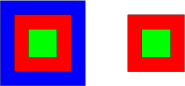
\includegraphics[width=0.5\textwidth]{sample3}
  \caption{En möjlig lösning till exempel 3.
  Till vänster en grön box är placerad i en röd box som är placerad i en blå box.
  Till höger en grön box placerad i en röd box.}
  \label{fig:sample3}
\end{figure}

Skriv ett program som givet boxarna säger vilken färgregel som ger minst antal
ytterboxar, och sedan skriver ut antalet ytterboxar det kommer bli.

\section*{Indata}

Indatan börjar med talet $N$, antalet boxar, där $1\le N \le 1\,000$. Därefter följer $N$ rader med sidlängd
$l_i$ ($1 \le l_i \le 10\,000\,000$) och färg $f_i$ (R, G, eller B) för varje box.

\section*{Utdata}

Totalt tre rader ska skrivas ut. Den första raden ska bestå av den första delen
av färgregeln, på formen ''$f_1$ i $f_2$'', medan den andra raden ska bestå av 
den andra delen av regeln, på formen ''$f_2$ i $f_3$''. Notera alltså att den sista bokstaven på
rad $1$ måste vara samma som den första bokstaven på rad $2$.
Den tredje och sista raden ska bestå av ett heltal, som beskriver antalet ytterboxar det kommer bli
efter man stoppat in dem i varandra. Om det finns mer än en färgregel 
som ger minimala antalet ytterboxar kan du skriva ut vilken som helst av dem.

\section*{Poängsättning}
Din lösning kommer att testas på en mängd testfallsgrupper. För att få poäng för en grupp
så måste du klara alla testfall i gruppen.

\noindent
\begin{tabular}{| l | l | l |}
\hline
% Grupp & Poängvärde & Gränser & Övrigt \\ \hline
Grupp & Poängvärde & Gränser \\ \hline
1     & 50         & Regeln kommer alltid att vara "R i G, G i B" \\ \hline
2     & 50         & Inga begränsningar. \\ \hline
\end{tabular}

\section*{Förklaring av exempel 3}
En möjlig lösning är illustrerad i Figur~\ref{fig:sample3}.
Vi kan lägga de två G-boxarna (storlek 1) i varsin R-box (storlek 10).
Därefter kan den ena R-boxen läggas i en B-box.
Kvar återstår då en R-box och en B-box som ytterboxar.
